\chapter{群速度、フェルミオン的排他、ディラックの海}

\section{位相速度と群速度}

\begin{classroomqa}
\lecturetimestamp{00:00:07}
\audiencequestion{群速度と位相速度とは何か。}
\lecturerresponse{位相速度は平面波の位相が一定である点を追う。一般に、測定可能な物体の運動を表すものではない。群速度は波束の包絡線を追うものであり、粒子、信号、確率の流れに対応する速度である。}
\end{classroomqa}

平面波から始める。
\begin{equation}
\psi(x,t)=e^{i(kx-\omega t)},
\end{equation}
またはその実形式から始める。
\begin{equation}
\psi(x,t)=\sin(kx-\omega t).
\end{equation}
山、谷、その他位相が一定の任意の点は、
\begin{equation}
kx-\omega t=\text{constant}.
\end{equation}
となるように動く。便宜上、定数をゼロと選べば、
\begin{equation}
x=\frac{\omega}{k}t,
\qquad
v_{\mathrm{phase}}=\frac{\omega}{k}.
\end{equation}
が得られる。\(\omega=2\pi/T\) かつ \(k=2\pi/\lambda\) であるから、
\begin{equation}
v_{\mathrm{phase}}=\frac{\omega}{k}=\frac{\lambda}{T}.
\end{equation}
これは、ある与えられた位相が一周期の間に進む距離にほかならない。

非相対論的な Schr\"odinger 波について、\(\hbar=1\) とすると、エネルギーと運動量は \(\omega\) および \(k\) であるから、
\begin{equation}
\omega(k)=\frac{k^2}{2m}.
\end{equation}
したがって、その位相速度は
\begin{equation}
v_{\mathrm{phase}}=\frac{k}{2m}.
\end{equation}
である。しかし、運動量 \(k\) をもつ粒子の通常の速度は \(k/m\) である。この2倍の不一致は、平面波の位相の動きが粒子の動きではないことを示す最初の警告である。

さらに鋭い警告がある。すべての振動数に同じ定数 \(C\) を加える。
\begin{equation}
\omega(k)\longrightarrow \omega(k)+C.
\end{equation}
この定数は、例えば \(mc_{\mathrm{light}}^2\) のような共通の静止エネルギー寄与を表すこともできるが、その具体的な名称は重要ではない。ここで \(C\) はエネルギーのオフセットであり、光速ではない。位相速度は
\begin{equation}
v_{\mathrm{phase}}\longrightarrow
\frac{\omega(k)+C}{k}
=v_{\mathrm{phase}}+\frac{C}{k}.
\end{equation}
に変わる。しかし、すべてのエネルギーに同じ定数を加えてもエネルギー差は変わらず、したがって非相対論的な物理は何も変わらない。

これは波動関数に直接見ることができる。一般の Schr\"odinger 場をモードの和または積分として書く。
\begin{equation}
\psi(x,t)=\sum_k a_k e^{ikx}e^{-i\omega(k)t},
\end{equation}
ここで規格化因子は省略した。シフトの後、
\begin{align}
\psi(x,t)
&\longrightarrow
\sum_k a_k e^{ikx}e^{-i[\omega(k)+C]t}
\\
&=e^{-iCt}\psi(x,t).
\end{align}
すべてのモードが同じ時間依存の位相を獲得した。共役場は逆の位相を獲得するので、
\begin{equation}
\begin{aligned}
\psi^*(x,t)\psi(x,t)
&\longrightarrow
e^{iCt}e^{-iCt}\psi^*(x,t)\psi(x,t)
\\
&=\psi^*(x,t)\psi(x,t).
\end{aligned}
\end{equation}
期待値でも同じ相殺が起こる。エネルギーの原点をずらすと変化する量は、Schr\"odinger 粒子の物理的な伝播速度ではありえない。したがって、位相速度は部分的に約束事である。

局在した粒子は、無限に広がる一つの平面波ではなく、波束によって表される。成分波は波束の領域では建設的に干渉し、その外側では破壊的に干渉する。このパターンの運動は、すでに近接する二つの波から求めることができる：
\begin{equation}
\psi(x,t)=
\sin(kx-\omega t)+
\sin(k'x-\omega't),
\end{equation}
ここで\(k'\)は\(k\)に近く、\(\omega'=\omega(k')\)である。建設的干渉の軌跡は、それらの位相が一致する場所に生じ、
\begin{equation}
kx-\omega t=k'x-\omega't.
\end{equation}
したがって
\begin{equation}
(k-k')x=(\omega-\omega')t,
\end{equation}
となり、強め合うパターンは次に従って移動する：
\begin{equation}
x=\frac{\omega-\omega'}{k-k'}t.
\end{equation}
隣接波の極限を取ると、
\begin{equation}
x=\frac{d\omega}{dk}t,
\qquad
v_{\mathrm{group}}=\frac{d\omega}{dk}.
\end{equation}
が得られる。これは包絡線---成分波の干渉によって生じた局在した塊の速度である。

非相対論的な分散関係について、任意のオフセットを含めると、
\begin{equation}
\omega(k)=\frac{k^2}{2m}+C,
\end{equation}
群速度は
\begin{equation}
v_{\mathrm{group}}
=\frac{d}{dk}\left(\frac{k^2}{2m}+C\right)
=\frac{2k}{2m}
=\frac{k}{m}.
\end{equation}
である。付加的な定数は消え、結果はまさに古典的な粒子速度である。

\begin{classroomqa}
\lecturetimestamp{00:16:35}
\audiencequestion{2の因子は群速度では消えるのか。}
\lecturerresponse{はい。\(k^2\) を微分すると \(2k\) が得られ、これが \(2m\) の2を打ち消す。結果は \(k/m\) である。}
\end{classroomqa}

したがって、群速度は古典的な粒子の運動に最も密接に関連する速度である。また、波束の伝播に関係する速度であり、ここで考える通常の状況では信号の伝播にも関係する。位相速度は、どちらの意味ももつ必要はない。

\subsection{質量ゼロおよび質量をもつ相対論的波}

\begin{classroomqa}
\lecturetimestamp{00:17:47}
\audiencequestion{これは光が光より速く進むことができるという主張と関係があるのか。}
\lecturerresponse{いいえ。それらの主張は別の問題を提起する。関連する計算は、物理的な群速度が光速以下にとどまる一方で位相が光より速く動きうることを確かに示すが、それは信号が光を追い越すことを表すものではない。}
\end{classroomqa}

\begin{classroomqa}
\lecturetimestamp{00:18:05}
\audiencequestion{関連する例は、位相速度が光速を超える一方で群速度が光速未満にとどまる、よく知られた例か。}
\lecturerresponse{はい。同じパターンは質量が非零の相対論的波にも現れ、それは相対論的なエネルギー--運動量関係から直接従う。}
\end{classroomqa}

\(\hbar=c_{\mathrm{light}}=1\)とおく。相対論的関係は
\begin{equation}
E=\sqrt{p^2+m^2},
\qquad
\omega(k)=\sqrt{k^2+m^2}.
\end{equation}
である。まず質量ゼロの場合を確立しておくと有用である。\(m=0\)のとき、
\begin{equation}
\omega=|k|.
\end{equation}
右向きに進む分枝\(k>0\)では\(\omega=k\)であり、したがって
\begin{equation}
v_{\mathrm{phase}}=\frac{\omega}{k}=1,
\qquad
v_{\mathrm{group}}=\frac{d\omega}{dk}=1.
\end{equation}
である。左向きに進む分枝では、両方の速度が対応する負の符号をもつ。いずれの場合もそれらの速さは光速である。分散関係がどちらの分枝でも線形であるため、その分枝上のすべてのフーリエ成分は同じ速度で動く。

\(k>0\)をもつ質量のある粒子に対しては、
\begin{equation}
v_{\mathrm{phase}}
=\frac{\omega}{k}
=\sqrt{\frac{k^2+m^2}{k^2}}>1,
\end{equation}
であるのに対し、
\begin{equation}
v_{\mathrm{group}}
=\frac{d\omega}{dk}
=\frac{k}{\sqrt{k^2+m^2}}<1.
\end{equation}
である。\(k<0\)では、両方の速度の符号が反転するが、それらの大きさは同じ不等式に従う。したがって、位相は光より速く動きうる一方で、波束、粒子、エネルギー、信号は光より遅く動く。この特定の分散関係と\(k\neq0\)に対しては、
\begin{equation}
v_{\mathrm{phase}}v_{\mathrm{group}}=1.
\end{equation}
である。この逆関係は平方根型分散関係の偶然であって、波の一般的な性質ではない。

\begin{figure}
\centering
\includegraphics[width=0.72\textwidth]{lecture_05_figure_03.png}
\caption{非相対論的および相対論的分散関係。位相速度\(\omega/k\)および群速度\(d\omega/dk\)。}
\lectureframe{00:35:52}
\end{figure}

\begin{classroomqa}
\lecturetimestamp{00:23:41}
\audiencequestion{分散は、波の速度が振動数に依存することと結びついているのですか。}
\lecturerresponse{はい。\(\omega(k)\)が線形であるとき、すべてのフーリエ成分は同じ群速度をもち、波束はその形を保つことができる。\(\omega(k)\)が非線形であるとき、異なる成分は異なる速度で動くので、波束は分散して形を変える。低振動数の音は、その振動数が波数にほぼ比例するとき、近似的に非分散である。}
\end{classroomqa}

位相速度は通常、信号もエネルギーも確率の流れも運ばない。その数値は、エネルギーの零点をずらすことによってさえ変わりうる。群速度は、十分に狭い波束の物理的に意味のある運動である。

\begin{classroomqa}
\lecturetimestamp{00:25:14}
\audiencequestion{光子について位相速度を測定することはできますか。}
\lecturerresponse{真空中では光子は線形な分散をもつので、その位相速度と群速度は一致し、どちらも光速に等しい。物質媒質中では分散関係が変わり、位相速度と群速度は一致する必要はない。}
\end{classroomqa}

\begin{classroomqa}
\lecturetimestamp{00:25:50}
\audiencequestion{この議論は、時間とともに広がらない波束に限られているのですか。}
\lecturerresponse{波束が広がらずにとどまるのは、そのすべてのフーリエ成分が一つの速度を共有する場合だけであり、それは関係する範囲で線形な分散関係に対応する。非線形な分散では成分が分離し、波束は広がる。}
\end{classroomqa}

光円錐と相対論的因果構造に関する問いは、位相速度と群速度の区別以上のものを必要とし、この計算とは別に扱う。

\section{並進対称性と保存則}

同じ平面波の位相が、保存則の簡潔な説明を与える。まずエネルギー保存から始める。エネルギー\(\omega_j\)の入射粒子に作用する消滅場は、時間因子
\begin{equation}
e^{-i\omega_j t},
\end{equation}
を与えるのに対し、エネルギー\(\omega'_r\)の出射粒子を生成する生成場は、
\begin{equation}
e^{+i\omega'_r t}.
\end{equation}
を与える。複数の入射粒子と出射粒子に対しては、それらの積は
\begin{equation}
\exp\!\left[
i\left(\sum_r\omega'_r-\sum_j\omega_j\right)t
\right].
\end{equation}
である。相互作用が同じ振幅で任意の時刻に起こりうるならば、振幅には相互作用時間にわたる積分が含まれる：
\begin{equation}
\begin{aligned}
&\int_{-\infty}^{\infty}dt\,
\exp\!\left[
i\left(\sum_r\omega'_r-\sum_j\omega_j\right)t
\right]
\\
&\quad =2\pi\,
\delta\!\left(\sum_r\omega'_r-\sum_j\omega_j\right).
\end{aligned}
\end{equation}
デルタ関数は、出射エネルギーの総和が入射エネルギーの総和に等しいことを要求する。あらゆる可能な相互作用時刻で振幅が等しいことは時間並進不変性であり、それがエネルギー保存を生み出す。

空間並進は、同じ仕組みによって運動量保存を与える。運動量\(k\)の入射粒子が消え、運動量\(k'_1\)と\(k'_2\)の2つの粒子が現れる物理的な1→2崩壊を考える。位置\(x\)における局所相互作用は、1つの消滅場と2つの生成場を含む。
\begin{equation}
\mathcal{O}(x)=\psi^\dagger(x)\psi^\dagger(x)\psi(x).
\end{equation}
時間依存性と規格化を省略すると、関係するモード因子は
\begin{align}
\psi(x)&\supset a_k e^{ikx},
\\
\psi^\dagger(x)&\supset a_{k'_1}^\dagger e^{-ik'_1x},
\qquad
\psi^\dagger(x)\supset a_{k'_2}^\dagger e^{-ik'_2x}.
\end{align}
である。行列要素
\begin{equation}
\langle k'_1,k'_2|\mathcal{O}(x)|k\rangle,
\end{equation}
において、消滅演算子は入射粒子を取り除き、2つの生成演算子は出射粒子を与える。これらの演算子の作用を取った後に残る位置依存因子は
\begin{equation}
e^{-ik'_1x}e^{-ik'_2x}e^{ikx}
=e^{i(k-k'_1-k'_2)x}.
\end{equation}
である。どの位置も特権的ではないので、可能なすべての崩壊位置について積分する：
\begin{equation}
\int_{-\infty}^{\infty}dx\,
e^{i(k-k'_1-k'_2)x}
=2\pi\delta(k-k'_1-k'_2).
\end{equation}
したがって、生き残る振幅は
\begin{equation}
k=k'_1+k'_2.
\end{equation}
に従う。3次元では、同じ計算は\(d^3x\)、太字の運動量ベクトル、および3次元デルタ関数を用いる。この議論のどこにも、入射粒子が1つだけであることや出射粒子が2つであることに依存する点はない。任意の粒子数に対して、共通の相互作用位置についての積分は
\begin{equation}
\delta^{(3)}\!\left(
\sum_j\mathbf{k}_j-\sum_r\mathbf{k}'_r
\right).
\end{equation}
を与える。すべての位置で振幅が等しいことは空間並進不変性であり、すべての時間で振幅が等しいことがエネルギー保存を与えるのとちょうど同じように、運動量保存を与える。

第3の例は大域的位相回転である：
\begin{equation}
\psi\longrightarrow e^{i\lambda}\psi,
\qquad
\psi^\dagger\longrightarrow e^{-i\lambda}\psi^\dagger.
\end{equation}
相互作用振幅は、その消滅場と生成場が寄与する位相が相殺するときに不変である。電荷を運ぶ場に対して、初期状態から取り除かれた電荷と最終状態で復元された電荷が等しいことは、電荷保存である。このように、時間並進、空間並進、および大域的位相回転は、粒子を生成・消滅させる場がエネルギー、運動量、および電荷の保存をどのように符号化するかを例示している。

\begin{classroomqa}
\lecturetimestamp{00:37:52}
\audiencequestion{空間についての積分とは、3つの空間次元すべてについての積分を意味するのですか。}
\lecturerresponse{はい。3つの積分は3つの運動量成分に対するデルタ関数を生じるので、全運動量の3つの成分すべてが保存されます。}
\end{classroomqa}

\begin{classroomqa}
\lecturetimestamp{00:38:03}
\audiencequestion{この模型は、保存された運動量を分け合う異なる仕方に対する相対確率を決定するのですか。}
\lecturerresponse{いいえ。この単純な表式は出射運動量の和を強制しますが、それ以外にはそれらの分配について中立です。相対確率には追加の動力学的情報が必要です。}
\end{classroomqa}

\begin{classroomqa}
\lecturetimestamp{00:39:04}
\audiencequestion{なぜ消滅演算子の和は、占有された運動量に一致する項に帰着するのですか。}
\lecturerresponse{空のモードに作用する消滅演算子はゼロベクトルを与えます。状態がモード\(k_0\)にのみ1つの粒子を含むなら、\(k=k_0\)をもつ項以外のすべての項は消えます。}
\end{classroomqa}

例えば、
\begin{equation}
\sum_k a_k e^{ikx}|1_{k_0}\rangle
=e^{ik_0x}|0\rangle,
\end{equation}
規格化を除いて、空のモードに対応するすべての消滅演算子はゼロベクトルを返す。

\section{ボソン的増強とフェルミオン的排他}

ボソンは1粒子状態において任意の非負の占有数を許し、その生成演算子代数は実際にすでに占有された状態を優遇する。1つのボソンモードに対して、規格化された数状態の慣例は占有増強を次のように書く\footnote{講義では平方根の占有増強が述べられている；この添字付き方程式はその標準的な数状態の形である。}
\begin{equation}
a^\dagger|n\rangle=\sqrt{n+1}\,|n+1\rangle.
\end{equation}
励起原子が多くの可能なモードへ光子を放出できるとする。他の光子が存在しない場合、異なる方向と運動量は通常の確率分布で生じる。もし特定のモードがすでに多くの光子を含み---それらはすべて同じ運動量、エネルギー、振動数をもつ---、そのモードへの放出は対応する平方根の占有因子によって増強される。原子はその光子を、すでに占有されている状態に優先的に加える。これが誘導放出であり、ボソンの集合性の具体的な表れである。

フェルミオンは逆に振る舞う。2つの同一なフェルミオンは同じ量子状態を占めることができない。排他原理はもともと原子物理学で生じた。そこでは原子内の2つの電子が同一の量子数をもつことができないが、それは原子に限定されない：同一なフェルミオンはどこでも完全な1粒子状態を共有することができない。

場の展開は最初はボソンの場合とまったく同じに見える。有限の箱では次のように書ける
\begin{equation}
\psi(x)=\sum_k A_k e^{ikx},
\qquad
\psi^\dagger(x)=\sum_k A_k^\dagger e^{-ikx}.
\end{equation}
連続的な運動量に対しては和が積分になる。共役な空間位相における逆符号はエルミート共役から従う。構成のこの部分は非相対論的である；相対論的フェルミオンは最後にのみ登場する。

場の状態は依然として各モードごとの占有数によって記録されるが、今や各数はゼロか一しか取り得ない：
\begin{equation}
|n_{k_1},n_{k_2},\ldots\rangle,
\qquad n_k\in\{0,1\}.
\end{equation}
例えば一状態あたり高々三粒子、あるいは一状態あたり少なくとも七粒子といった、追加の相対論的粒子種は存在しない。ボソン統計とフェルミオン統計が唯一の可能性であることを確立するには、量子力学と特殊相対性理論が必要であり、本稿の範囲を超えている。ここでの課題は、フェルミオン的可能性とその帰結を記述することである。

\subsection{一つのフェルミオン状態}

単一の1粒子状態に注目する。それは空であるか、\(|0\rangle\)、あるいは占有されているか、\(|1\rangle\)、のいずれかである。生成と消滅は次のように作用する：
\begin{align}
A^\dagger|0\rangle&=|1\rangle,
&
A^\dagger|1\rangle&=0,
\\
A|0\rangle&=0,
&
A|1\rangle&=|0\rangle.
\end{align}
右辺の装飾のないゼロは零ベクトルであり、空状態\(|0\rangle\)ではない。2番目のフェルミオンを加えようとしても真空に戻るのではなく、物理的状態が全く得られない。

\begin{classroomqa}
\lecturetimestamp{00:46:25}
\audiencequestion{フェルミオンの生成・消滅演算子もやはり線形か？}
\lecturerresponse{はい。量子力学の演算子は線形演算子であり、フェルミオンの生成・消滅演算子も含まれる。}
\end{classroomqa}

\begin{classroomqa}
\lecturetimestamp{00:47:34}
\audiencequestion{ゼロとは空状態を意味するのか、それとも試みた操作が状態を生成できないことを意味するのか？}
\lecturerresponse{それは零ベクトルを意味し、空状態ではない。真の真空または基底状態は非零の波動関数を持ち、恒等的にゼロの関数はノルムがゼロであり、物理的状態ではない。}
\end{classroomqa}

調和振動子はこの区別を具体的にする。その基底状態、すなわち振動子の励起がない状態は、次のようなガウス型波動関数を持つ：
\begin{equation}
\phi_0(q)\propto e^{-\alpha q^2},
\qquad \alpha>0.
\end{equation}
これは完全に良好で規格化可能な状態である。対照的に、
\begin{equation}
\phi(q)\equiv0
\end{equation}
は零ベクトルである：どこにも確率振幅を持たず、状態ではない。したがって\(A^\dagger|1\rangle=0\)は、試みられた2番目の生成が零ベクトルを生み出すことを述べている。

\begin{classroomqa}
\lecturetimestamp{00:48:42}
\audiencequestion{フェルミオン演算子はボソン演算子と異なる記法を使うべきか？}
\lecturerresponse{はい。\(a\)と\(a^\dagger\)はボソンモード用に確保し、\(c\)と\(c^\dagger\)をフェルミオンモード用に使う方が明確である。両方の慣習が文献にあるが、異なる文字を使うことで二つの代数が区別される。}
\end{classroomqa}

その記法を採用すると、単一モードの規則は次のようになる：
\begin{align}
c^\dagger|0\rangle&=|1\rangle,
&c^\dagger|1\rangle&=0,
\\
c|0\rangle&=0,
&c|1\rangle&=|0\rangle.
\end{align}
次に、二つの基底状態に対する二つの可能な積を評価する。空状態では、
\begin{align}
c^\dagger c|0\rangle&=0,
&
cc^\dagger|0\rangle&=|0\rangle.
\end{align}
占有状態では、
\begin{align}
c^\dagger c|1\rangle&=|1\rangle,
&
cc^\dagger|1\rangle&=0.
\end{align}
それらの和は、作用する状態をそのまま返す：
\begin{align}
(c^\dagger c+cc^\dagger)|0\rangle&=|0\rangle,
\\
(c^\dagger c+cc^\dagger)|1\rangle&=|1\rangle.
\end{align}
\(|0\rangle\)と\(|1\rangle\)が1モードの状態空間を張るので、
\begin{equation}
c^\dagger c+cc^\dagger=1.
\end{equation}
プラス符号の組み合わせは反交換子であり、
\begin{equation}
\{A,B\}=AB+BA,
\end{equation}
したがってフェルミオンの関係は
\begin{equation}
\{c,c^\dagger\}=1.
\end{equation}
これはボソンの交換子
\begin{equation}
[a,a^\dagger]=aa^\dagger-a^\dagger a=1.
\end{equation}
のフェルミオン版である。

同じフェルミオン状態への2回の生成は常に消える。状態が空なら、最初の生成がそれを満たし、2番目は失敗する。すでに占有されていれば、最初の生成がすでに失敗する。同様に、2回の消滅は常に消える。したがって
\begin{equation}
\{c^\dagger,c^\dagger\}=2(c^\dagger)^2=0,
\qquad
\{c,c\}=2c^2=0.
\end{equation}

\begin{classroomqa}
\lecturetimestamp{00:56:45}
\audiencequestion{消滅の二乗の関係におけるゼロは零ベクトルか？}
\lecturerresponse{この方程式は\(c^2\)が零演算子であることを述べている。それはすべての状態ベクトルを零ベクトルに送る演算子である。零演算子と零ベクトルは異なる数学的対象であるが、前者は常に後者を生み出す。}
\end{classroomqa}

多くの離散的な運動量モードに対して、完全な代数は
\begin{align}
\{c_k,c_{k'}^\dagger\}&=\delta_{kk'},
\\
\{c_k,c_{k'}\}&=0,
\\
\{c_k^\dagger,c_{k'}^\dagger\}&=0.
\end{align}
クロネッカーのデルタは\(k=k'\)のとき1、それ以外では0である。連続的な運動量に対しては、適切な規格化とともにディラックのデルタ関数に置き換えられる。同種の反交換子は、ラベルが一致する場合だけでなく、あらゆるモードの対に対して消える。

\subsection{位置空間における排他}

運動量でラベル付けされた代数は、まず同じ種の2つの同一フェルミオンが一つの運動量モードを占めることはできないと述べている。それはさらに多くを述べている。位置\(x\)に局在する粒子は、規格化を除いて
\begin{equation}
\psi^\dagger(x)=\sum_k c_k^\dagger e^{-ikx},
\end{equation}
によって生成される。原点で2つの粒子を生成しようとすると、
\begin{align}
\psi^\dagger(0)\psi^\dagger(0)|\Omega\rangle
&=\sum_{k,k'}c_k^\dagger c_{k'}^\dagger|\Omega\rangle.
\end{align}
が得られる。ラベル\(k\)と\(k'\)はダミー和変数である。それらを交換しても二重和は変わらないので、ラベルを付け替えた形と平均してよい：
\begin{align}
\sum_{k,k'}c_k^\dagger c_{k'}^\dagger|\Omega\rangle
&=\frac12\sum_{k,k'}
\left(c_k^\dagger c_{k'}^\dagger
+c_{k'}^\dagger c_k^\dagger\right)|\Omega\rangle
\\
&=\frac12\sum_{k,k'}
\{c_k^\dagger,c_{k'}^\dagger\}|\Omega\rangle
=0.
\end{align}

\begin{classroomqa}
\lecturetimestamp{01:02:26}
\audiencequestion{2粒子位置状態の和で消えるのは運動量が等しくない項だけか？}
\lecturerresponse{いいえ。ダミー添字を付け替えると、二重和全体が2つの生成演算子の反交換子の半分になる。その反交換子はあらゆる運動量の対に対して消えるので、和全体はゼロである。}
\end{classroomqa}

この計算は、排他性が運動量固有状態に特有のものではないことを示している。同種のフェルミオンは同じ位置状態に置くこともできない。より一般には、同一の一粒子状態を占めることはできない。

\subsection{何が同じ状態を構成するのか？}

\begin{classroomqa}
\lecturetimestamp{01:04:30}
\audiencequestion{遠く離れた2つの電子が同じ運動量をもつことはあり得るか？}
\lecturerresponse{排他性が関わるのは完全な一粒子状態である。2つの電子は、スピンのような別の可換なラベルが異なっていれば、同じ正確な運動量固有値をもつことができる。空間的に離れた電子はむしろ局在した波束であり、正確な運動量固有状態ではない。それらの平均運動量はほぼ等しくても、空間波動関数は異なったままであり得る。禁じられているのは、完全な状態が等しいことである。}
\end{classroomqa}

スピンはまだ展開されていないが、よく知られた追加のラベルを与える。2つの電子は、スピン状態が異なっていれば、同じ運動量の値を共有できる。関係するすべてのラベルを含めれば、2つの同種フェルミオンが同じ完全な状態を共有することはできない。

\begin{classroomqa}
\lecturetimestamp{01:05:25}
\audiencequestion{離れた2つの水素原子中の電子が同じ運動量または原子状態をもつことはあり得るか？}
\lecturerresponse{原子に束縛された電子は運動量固有状態ではない。その軌道波動関数はその原子を中心としている。離れた2つの原子がそれぞれ原子基底状態と呼ばれる状態の電子をもつことはあり得るが、一方の軌道は第1の原子を中心とし、他方は第2の原子を中心とするので、それらは異なる一粒子状態である。}
\end{classroomqa}

\begin{classroomqa}
\lecturetimestamp{01:06:33}
\audiencequestion{より一般的な語である系が状態に代わり得るか？}
\lecturerresponse{いいえ。系とは自由度の集まりであり、状態とはその系の特定の量子配置を指定するものである。電子は系であり、その軌道およびスピン波動関数はその系の状態を記述する。}
\end{classroomqa}

\begin{figure}
\centering
\includegraphics[width=0.74\textwidth]{lecture_05_figure_04.png}
\caption{局在した一粒子波動関数と、フェルミオン的排他性を検証するために用いられる2生成演算子状態。}
\lectureframe{01:07:21}
\end{figure}

\begin{classroomqa}
\lecturetimestamp{01:07:22}
\audiencequestion{陰極線管内の電子流には、同じ状態にある2つの電子が存在しないのか？}
\lecturerresponse{はい。電子は、位置的に分離されるか、あるいは完全な状態において別様に区別される、異なる波束を占める。これは、すべてが同じ平面波モードを占めてコヒーレントなビームを形成し得る光子とは対照的である。}
\end{classroomqa}

電子ビームは、1つの局在した波束の後に別の波束が続くものとして描くことができる。波束は正確な位置状態や正確な運動量状態である必要はなく、それらの波動関数が異なっていれば十分である。対照的に、光子ビームでは、多くの光子がまったく同じ平面波状態にあってもよい。

\begin{classroomqa}
\lecturetimestamp{01:08:14}
\audiencequestion{2つの電子が異なる運動量をもって同じ位置に存在することはあり得るか？}
\lecturerresponse{正確な位置と正確な運動量は、対応する演算子が可換でないため、両立しないラベルである。位置と運動量を同時に鋭く指定して一粒子状態を定めることはできない。この非相対論的な設定ではスピンはそれらの可観測量と可換であるため、スピンは位置または運動量のラベルに付随し得る。}
\end{classroomqa}

\begin{classroomqa}
\lecturetimestamp{01:08:51}
\audiencequestion{離れた束縛電子は近似的に位置状態にあるのか？}
\lecturerresponse{それらは正確な位置固有状態ではない。各軌道は有限の空間的広がりをもつからである。しかし各電子はそれぞれ自身の原子の近くに近似的に局在している。その局在性は、2つの軌道波動関数を異なる状態とするのに十分である。}
\end{classroomqa}

\begin{classroomqa}
\lecturetimestamp{01:09:31}
\audiencequestion{量子状態の定義とは何か？}
\lecturerresponse{状態とは、系の配置の量子力学的な類似物である。それは、可能な測定に確率を割り当てるために必要な情報を含む。1つの電子については、状態は波動関数によって表され、スピンのような内部ラベルがあればそれも伴う。}
\end{classroomqa}

\begin{classroomqa}
\lecturetimestamp{01:10:32}
\audiencequestion{非常に遠く離れた場所に局在する電子が同じ状態にあること、または同じ運動量をもつことはあり得るか？}
\lecturerresponse{それらは同じ状態ではあり得ない。局在の仕方が異なるからである。ここにある電子とアンドロメダ銀河にある電子、あるいはネバダにある電子とコネチカットにある電子は、異なる波動関数をもつ。それらはほぼ等しい運動量をもち得る。どちらかの運動量を無限に鋭くすると、対応する波動関数が空間全体に広がり、状態を区別していた局在性が破壊されてしまう。}
\end{classroomqa}

位置--運動量の不確定性関係の標準偏差形は\footnote{講義では不確定性積に関する定性的な記述が与えられており、因子\(\hbar/2\)は標準偏差の慣習で補われている。}
\begin{equation}
\Delta x\,\Delta p\geq\frac{\hbar}{2}.
\end{equation}
ある波束はネバダに局在し、かなり狭い運動量分布を持ちうるが、コネチカットにある別の波束はほぼ同じ分布を持つ。それらは空間的波動関数が異なるため、異なる状態であり続ける。厳密な運動量固有状態の極限では、どちらの波束もどちらの場所にも局在したままではない。

フェルミオン演算子は、ボソン演算子と同様の仕方で反応に用いられる。電子の消滅演算子は入射電子を取り除き、電子の生成演算子は出射電子を供給し、これらの因子は光子の生成演算子または消滅演算子と掛け合わされうる。光子はボソンであり、電子はフェルミオンである。それらの演算子の積は、入射電子と出射電子および放出または吸収される光子を含む反応の勘定を与える。

\begin{classroomqa}
\lecturetimestamp{01:13:36}
\audiencequestion{パウリ排他は局所的に伝達されるのか、それとも二つの生成過程が空間的に離れているときに大域的に強制されるのか。}
\lecturerresponse{一方の粒子がネバダにあり、他方がコネチカットにあると分かっているなら、それらは同じ状態にはない。}
\end{classroomqa}

\editorialnote{この問いへの回答の短い部分は復元できない。局在した一粒子状態とネバダ--コネチカットの重ね合わせとの区別は確かなものである。}

それらの位置が確定していないとき、排他は完全な一粒子波動関数が一致するかどうかを問う。ネバダ--コネチカットの重ね合わせはその区別を明示する。

\(|N\rangle\)と\(|C\rangle\)を、ネバダとコネチカットに局在する正規直交状態とする。このとき
\begin{equation}
|+\rangle=\frac{|N\rangle+|C\rangle}{\sqrt2},
\qquad
|-\rangle=\frac{|N\rangle-|C\rangle}{\sqrt2}.
\end{equation}
状態\(|+\rangle\)は、その一つの電子がネバダまたはコネチカットに見出される等しい確率を与える。状態\(|-\rangle\)は同じ位置確率を与えるが、相対位相だけが異なる。この二つの状態は直交する：
\begin{equation}
\langle+|-\rangle=0.
\end{equation}
二つの電子はともに\(|+\rangle\)を占めることはできず、ともに\(|-\rangle\)を占めることもできないが、排他は一方の電子が各状態を一つずつ占めることを妨げない。

\begin{classroomqa}
\lecturetimestamp{01:16:25}
\audiencequestion{一方の電子がプラスのネバダ--コネチカット重ね合わせを占め、他方がマイナスの重ね合わせを占めることはできるか。}
\lecturerresponse{できる。プラスとマイナスの組み合わせは直交し、したがって異なる一粒子状態である。}
\end{classroomqa}

\begin{classroomqa}
\lecturetimestamp{01:16:39}
\audiencequestion{分離した状態の例には同時性の概念が必要か。}
\lecturerresponse{現在の模型は非相対論的である。それは、空間的に離れたネバダとコネチカットの領域が共有する絶対時間のもとで、一つの共通の時間スライス上で二つの占有状態を比較する。また、それらの領域を比較する際の有限速度の操作上の制限を無視している。相対論的物理学は、粒子がどのように局在するかにさらなる曖昧さをもたらすが、排他を無効にはしない。ただし、その精密化はここでは後回しにされる。}
\end{classroomqa}

本質的な非相対論的記述は今や確定した。フェルミオンは反交換する生成演算子と消滅演算子によって記述され、二つの同一なフェルミオンが一つの完全な一粒子状態を占めることはできない。したがって多体基底状態はボソンのそれとは根本的に異なる。

\section{有限箱の中のボソン基底状態とフェルミオン基底状態}

一辺\(L\)の有限な三次元箱に閉じ込められ、周期的境界条件に従う粒子を考える。一次元では許される波数は
\begin{equation}
k=\frac{2\pi n}{L},
\qquad n\in\mathbb{Z}.
\end{equation}
三次元ではこの条件は成分ごとに適用される：
\begin{equation}
\mathbf{k}=\frac{2\pi}{L}(n_x,n_y,n_z),
\qquad n_x,n_y,n_z\in\mathbb{Z}.
\end{equation}
したがって許される運動量ベクトルは運動量空間内の格子をなす。これは位置の格子ではなく、各点が許される運動量状態を表す。\(L\)を大きくすると隣り合う値の間隔\(2\pi/L\)は小さくなり、格子はあらゆる運動量方向に際限なく続く。

\begin{figure}
\centering
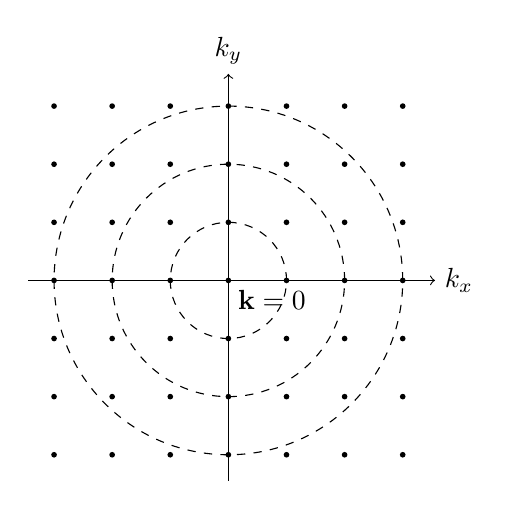
\begin{tikzpicture}[scale=0.82]
\draw[->] (-3.1,0) -- (3.2,0) node[right] {$k_x$};
\draw[->] (0,-3.1) -- (0,3.2) node[above] {$k_y$};
\draw[dashed] (0,0) circle (0.9);
\draw[dashed] (0,0) circle (1.8);
\draw[dashed] (0,0) circle (2.7);
\foreach \x in {-3,-2,-1,0,1,2,3}{
  \foreach \y in {-3,-2,-1,0,1,2,3}{
    \fill (0.9*\x,0.9*\y) circle (1.25pt);
  }
}
\node[below right] at (0,0) {$\mathbf{k}=0$};
\end{tikzpicture}
\caption{有限な周期的箱の中の粒子に対する離散的な運動量状態と等エネルギー殻。}
\end{figure}

非相対論的粒子に対して
\begin{equation}
E_{\mathbf{k}}=\frac{\mathbf{k}^2}{2m},
\end{equation}
であるから、最低エネルギーの状態は\(\mathbf{k}=0\)である。\(N\)個の同一なボソンを箱に入れ、多粒子基底状態を求める。最初のボソンはゼロ運動量状態に入る。二番目も同じ状態に入ることができ、三番目およびそれ以降のすべてのボソンも同様である。したがって\(N\)個のボソンすべてが\(\mathbf{k}=0\)を占める。

これはボース凝縮体である。多数の同一粒子が同じ一粒子状態、ここでは最低エネルギー状態を占めている。ゼロ運動量の波動関数は空間的に一定であり、箱全体に広がっている。それはいずれか一つのボース粒子を特定の位置に局在させるものではなく、それに対応して各ボース粒子は自分がどこにいるかについて不確定である。占有数が大きくなると、共通の波動関数が巨視的な場の振幅を築き上げ、場はますます古典場のように振る舞う。

フェルミオン基底状態は全く異なる。今はスピンを無視すると、各運動量点が一つの利用可能な状態を表す。最初のフェルミオンは\(\mathbf{k}=0\)に入るが、二番目の同一フェルミオンはそこに加わることはできない。次の粒子は次に低いエネルギーの殻を占めなければならない。二次元の図では、等しいエネルギーの最近接の非零格子点が四つあり、三次元では六つある。それらの状態が占められた後、さらに粒子は successive な殻へと入らなければならない。

エネルギーは運動量空間における原点からの距離の二乗に比例するので、全エネルギーを最小化することは、排他律が許す限り占められた点を\(\mathbf{k}=0\)の周りにできるだけ密に詰めることを意味する。多数のフェルミオンがあると、占有領域は球に近づく。その境界がフェルミ面であり、内部がフェルミ海であり、完全に満たされた領域がフェルミ球である。有限体積では、利用可能な点が格子を形成するため境界はわずかにぎざぎざになるが、この細部は大きな系では無視できるようになる。

\begin{figure}
\centering
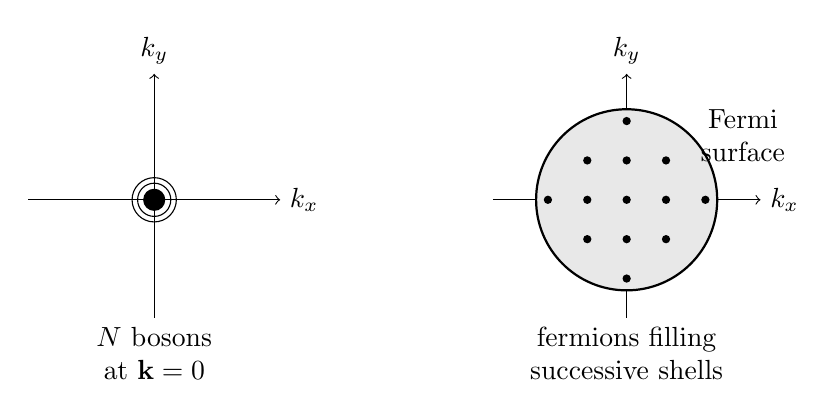
\begin{tikzpicture}[scale=1.0]
\begin{scope}[xshift=-3.0cm]
\draw[->] (-1.6,0) -- (1.6,0) node[right] {$k_x$};
\draw[->] (0,-1.5) -- (0,1.6) node[above] {$k_y$};
\fill (0,0) circle (4pt);
\draw (0,0) circle (6pt);
\draw (0,0) circle (8pt);
\node[align=center] at (0,-1.95) {$N$ bosons\\at $\mathbf{k}=0$};
\end{scope}
\begin{scope}[xshift=3.0cm]
\draw[->] (-1.7,0) -- (1.7,0) node[right] {$k_x$};
\draw[->] (0,-1.5) -- (0,1.6) node[above] {$k_y$};
\fill[gray!18] (0,0) circle (1.15);
\draw[thick] (0,0) circle (1.15);
\fill (0,0) circle (1.5pt);
\fill (0.5,0) circle (1.5pt);
\fill (-0.5,0) circle (1.5pt);
\fill (0,0.5) circle (1.5pt);
\fill (0,-0.5) circle (1.5pt);
\fill (0.5,0.5) circle (1.5pt);
\fill (0.5,-0.5) circle (1.5pt);
\fill (-0.5,0.5) circle (1.5pt);
\fill (-0.5,-0.5) circle (1.5pt);
\fill (1,0) circle (1.5pt);
\fill (-1,0) circle (1.5pt);
\fill (0,1) circle (1.5pt);
\fill (0,-1) circle (1.5pt);
\node[right,align=center] at (0.82,0.82) {Fermi\\surface};
\node[align=center] at (0,-1.95) {fermions filling\\successive shells};
\end{scope}
\end{tikzpicture}
\caption{ボース粒子はゼロ運動量状態に凝縮するのに対し、フェルミ粒子はフェルミ面まで外側へ運動量状態を満たす。}
\end{figure}

フェルミオン基底状態は、対応するボース基底状態よりもはるかに多くのエネルギーを持つ。すべてのボース粒子はゼロ運動量にとどまることができるが、フェルミ粒子の大部分は非零運動量状態へと強いられる。フェルミ粒子がさらに加えられると、占められる最大運動量が増大する。さらに、大きな運動量の殻は原点近くの殻よりも多くの格子点を含む。したがって大きなフェルミ球は、かなりの運動量を持つ多数の粒子を含み、最低運動量状態には少数の粒子しか含まない。

この対比は励起状態でも続く。ボース粒子の場合、最初の励起は任意の一つのボース粒子を凝縮体から取り除き、それを第一励起一粒子状態に置くことによって得られる：
\begin{equation}
(N,0,0,\ldots)\longrightarrow (N-1,1,0,\ldots).
\end{equation}
どのボース粒子を動かすかは違いを生まない。粒子は同一である。より高い励起はいくつかの方法で作ることができる。準位間隔に応じて、一つのボース粒子をより高い準位に置くか、二つのボース粒子を第一励起準位に置くことができる。ボース系を励起することは、粒子を凝縮体からより高いエネルギー状態へと昇進させることを意味する。

フェルミ粒子の場合、満たされたフェルミ球の内部の別の点へ粒子を動かすことはできない。そのような点はすべてすでに占められているからである。海の深部からフェルミ粒子を取り出して表面の上に置くことは可能だが、大きなエネルギーを要する。最も低コストの励起は、フェルミ面のすぐ内側からフェルミ粒子を取り出し、すぐ外側の空いた状態へ動かすことである。昇進した電子は表面よりわずかに高いエネルギーしか持たず、残された空状態は表面よりわずかに低いエネルギーにある。

\begin{figure}
\centering
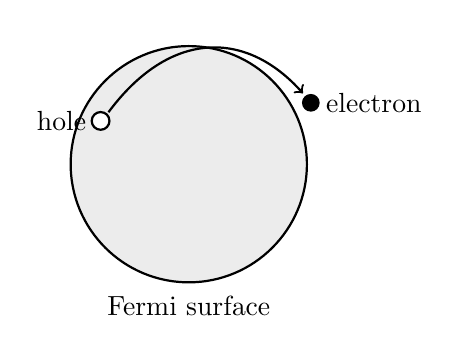
\begin{tikzpicture}[scale=1.0]
\fill[gray!15] (0,0) circle (1.5);
\draw[thick] (0,0) circle (1.5);
\draw[fill=white,thick] (-1.12,0.55) circle (3.2pt);
\fill (1.55,0.78) circle (3.2pt);
\draw[->,thick] (-1.02,0.66) .. controls (-0.25,1.7) and (0.72,1.72) .. (1.45,0.9);
\node[left] at (-1.18,0.55) {hole};
\node[right] at (1.62,0.78) {electron};
\node[below] at (0,-1.55) {Fermi surface};
\end{tikzpicture}
\caption{低エネルギーのフェルミオン励起は電子をフェルミ面を通して昇進させ、後に正孔を残す。}
\end{figure}

\section{正孔と低エネルギー励起}

正孔の電荷を具体的にするために、箱がその体積全体に一様に塗り広げられた正電荷を含んでいると想像しよう。物質ではその正電荷は最終的に原子核内の陽子に由来するが、一様分布はモデルを単純に保つ。背景を中性化するのに十分な電子を加える。基底状態ではそれらの電子がフェルミ球を満たす。

一つの電子をフェルミ面の下から上へ昇進させても、箱の全電荷は変化しない。それは表面の上に負に帯電した電子を生成し、その下に欠けた負電荷を残す。したがって欠けた電子は正に帯電した励起、すなわち正孔として扱うことができる。

\begin{classroomqa}
\lecturetimestamp{01:31:38}
\audiencequestion{フェルミ面の下の正孔は負のエネルギーを持つのか？}
\lecturerresponse{いいえ。正孔は多体基底状態の上の励起であるから、その励起エネルギーは正である。フェルミ面の下から占有された電子を取り除くことは、エネルギーをその面に対して測るとき、正の量のエネルギーを要する。}
\end{classroomqa}

取り除かれた電子のエネルギーを\(\varepsilon<\varepsilon_F\)とし、励起された電子のエネルギーを\(\varepsilon'>\varepsilon_F\)とする。供給されたエネルギーは、フェルミ面からの二つの正の距離に分けることができる。\footnote{二つの間隔は別々に述べられており、ここに示した簡潔な等式は代数的に等価な再構成である。}
\begin{equation}
\Delta E
=\varepsilon'-\varepsilon
=(\varepsilon'-\varepsilon_F)+(\varepsilon_F-\varepsilon).
\end{equation}
第一の寄与は自然にフェルミ面より上の電子に割り当てられ、第二の寄与はその下の正孔に割り当てられる：
\begin{equation}
E_{\mathrm{electron}}=\varepsilon'-\varepsilon_F>0,
\qquad
E_{\mathrm{hole}}=\varepsilon_F-\varepsilon>0.
\end{equation}
電子は負の電荷を運び、正孔は正の電荷を運ぶ。

フェルミ面より上の電子は、後に空いている正孔へ落ち込むことがある。そのときそのエネルギーは減少するので、放出されたエネルギーを放射が運び去らなければならない。この事象は、電子が空いている低い状態へ落ち込み、一つ以上の光子を放出すると記述できる。等価に、電子と正孔が対消滅して放射になると言うこともできる。正孔は箱の追加の基本的構成要素ではなく、満たされた多電子状態における欠如である。それにもかかわらず、そのエネルギーと電荷のため、粒子のような励起として扱うと便利である。

\begin{classroomqa}
\lecturetimestamp{01:36:52}
\audiencequestion{電子を励起するとは、運動量空間のある格子点から別の格子点へ動かすことを意味するのか？}
\lecturerresponse{それは電子をあるエネルギー準位から別のエネルギー準位へ動かすことを意味する。箱の中の自由粒子では、運動量格子がそれらの準位をラベル付けするが、同じ考えは運動量空間の格子に依存しない。原子では、正電荷は原子核に集中している。電子は利用可能な最も低い原子準位を満たし、光子は一つの電子を励起準位へ上げ、それが来た準位に空席を残すことができる。その空席が正孔の原子的対応物である。}
\end{classroomqa}

箱の中では、光子の吸収も同様に光子のエネルギーをフェルミ面より上の電子とその下の正孔に変換する。原子では、同じ言葉が励起電子と、占有された低い準位の間に残された空席を一緒に記述する。

\begin{classroomqa}
\lecturetimestamp{01:39:16}
\audiencequestion{低エネルギーの光子はフェルミ球内のどこにある電子にも吸収されうるか？}
\lecturerresponse{いいえ。電子がフェルミ海の深くにあるなら、近くのすべての状態はすでに占有されており、低エネルギーの光子はそれを表面より上の空いている状態まで持ち上げることはできない。光子のエネルギー範囲内で到達可能な空状態を持つのは、フェルミ面に十分近い電子だけである。十分にエネルギーの高い光子は、海の深くから電子を励起できる。}
\end{classroomqa}

したがって、低エネルギー吸収断面積はフェルミ海の全体積ではなく、その表面によって支配される。海の深くの電子は小さな遷移を行うことを妨げられ、表面のすぐ下の電子はそのすぐ上へ動かされうる。

\begin{classroomqa}
\lecturetimestamp{01:40:42}
\audiencequestion{入射光子なしで、電子が互いに直接相互作用することを何が妨げるのか？}
\lecturerresponse{何も妨げない。電子--電子相互作用はこの単純な模型では無視されている。それらを含めるとフェルミ海の描像がより複雑になるからである。金属へのこの第一近似では、それらの有効な影響は通常無視できるほど弱いものとして扱われる。}
\end{classroomqa}

\begin{classroomqa}
\lecturetimestamp{01:41:10}
\audiencequestion{一つの光子が複数の電子を励起するのに十分なエネルギーを運ぶとどうなるか？}
\lecturerresponse{保存則と整合するいかなる過程も原理的には可能である。光子は複数の電子--正孔対を生成できる：二つの電子を励起すれば二つの正孔も残る。そのような過程はより多くの励起を生成し、一般に、エネルギーを一つの電子をはるかに強く励起するために使う場合よりも確率が低い。}
\end{classroomqa}

\begin{classroomqa}
\lecturetimestamp{01:42:06}
\audiencequestion{どちらの光子も単独では励起を生成できないとき、二つの光子が一緒に吸収されうるか？}
\lecturerresponse{はい。吸収は確率的であり、二光子過程は、それぞれの光子が単独では必要なエネルギーを下回っていても、合わせた光子エネルギーが利用可能な励起に達するときに起こりうる。利用可能な光が許された励起に達するにはエネルギーが小さすぎる場合、それは主に系を通過する。}
\end{classroomqa}

\editorialnote{この時点での短い議論は、吸収された放射を集団的な電子運動と結びつけるが、その実質的な詳細は回復できない。そのような集団的応答が単一粒子--正孔描像よりも複雑であるという記述だけが確実である。}

\begin{classroomqa}
\lecturetimestamp{01:43:49}
\audiencequestion{すべての電子が同じ負電荷を帯びているのに、なぜ電子--電子相互作用は弱いと呼ばれるのか。}
\lecturerresponse{電子は補償する正の背景の中に浸されている。その背景が電子の電荷を遮蔽し、この簡略化された設定における有効相互作用を弱める。相互作用が存在しないわけではなく、それを扱うには媒質の遮蔽応答が必要である。}
\end{classroomqa}

\begin{classroomqa}
\lecturetimestamp{01:44:41}
\audiencequestion{遮蔽は後で議論されるのか。}
\lecturerresponse{はい。遮蔽は重要であるが、相互作用系をより完全に扱えるようになるまで延期される。}
\end{classroomqa}

\section{一次元フェルミオン海と反粒子}

空孔の構成は反粒子を指し示している。同じ論理構造は、物質中の電子から相対論的量子場とその真空へと移すことができる。最も単純な版では、一次元の空間と質量ゼロのフェルミオン場\(\psi(x,t)\)を用いる。光速度を1とする単位では、可能な2つの線形分散関係は
\begin{equation}
\omega=k,
\qquad\text{or}\qquad
\omega=-k.
\end{equation}
である。第1の分枝を明示的に考察する。

\editorialnote{最後のやり取りは、両立しない粒子の同定を交互に述べている。確実な模型は、一次元空間における、伝播の一方向に制限された、指定されていない質量ゼロのフェルミオン的トイ場である。}

平面波
\begin{equation}
\psi(x,t)=e^{i(kx-\omega t)},
\end{equation}
に対して、導関数は
\begin{equation}
\frac{\partial\psi}{\partial t}=-i\omega\psi,
\qquad
\frac{\partial\psi}{\partial x}=ik\psi.
\end{equation}
である。したがって\(\omega=k\)は、一次の場の方程式
\begin{equation}
\frac{\partial\psi}{\partial t}
=-\frac{\partial\psi}{\partial x}.
\end{equation}
と等価である。

\begin{figure}
\centering
\includegraphics[width=0.72\textwidth]{lecture_05_figure_05.png}
\caption{平面波が\(\omega=k\)を満たす一次の場の方程式を始める。}
\lectureframe{01:47:22}
\end{figure}

\(f(x-t)\)の形の任意のプロファイルはこの方程式を満たし、右へ移動する。符号を逆にすると
\begin{equation}
\frac{\partial\psi}{\partial t}
=+\frac{\partial\psi}{\partial x},
\end{equation}
となり、そのプロファイル\(f(x+t)\)は左へ移動する。どちらの一次の方程式も運動の一方向のみを選び出す。場をフェルミオン的とし、空孔の議論のために、その粒子が電荷を帯びていると仮定する。

分枝\(\omega=k\)には直ちに困難が伴う。波数\(k\)は負になり得るので、\(\omega\)も負になり得る。これらの単位では\(\omega\)がエネルギーであるから、直線的なスペクトルは正エネルギー状態と負エネルギー状態の両方を含む：
\begin{equation}
E=\omega=k.
\end{equation}

\begin{figure}
\centering
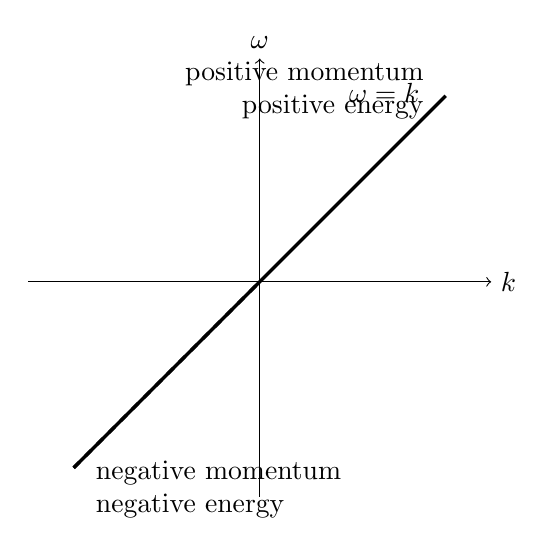
\begin{tikzpicture}[scale=1.05]
\draw[->] (-2.8,0) -- (2.8,0) node[right] {$k$};
\draw[->] (0,-2.6) -- (0,2.7) node[above] {$\omega$};
\draw[very thick] (-2.25,-2.25) -- (2.25,2.25);
\draw[very thick,dashed] (-2.25,-2.25) -- (0,0);
\node[above left] at (2.05,2.05) {$\omega=k$};
\node[below right,align=left] at (-2.1,-2.05) {negative momentum\\negative energy};
\node[above left,align=right] at (2.1,1.85) {positive momentum\\positive energy};
\end{tikzpicture}
\caption{一分枝スペクトル\(\omega=k\)と、\(k<0\)におけるその負エネルギーの半分。}
\end{figure}

通常の空の真空は、そのような理論の基底状態にはなり得ない。正エネルギーのフェルミオンは光子を放出してより低い状態へ落ち込むことができる。ゼロで止まることを強制するものは何もない。負エネルギーの状態へと進み続け、さらに多くの放射を放出し、際限なく落ち込むことができる。フェルミオンが失ったエネルギーは放射場に現れるであろう。したがって、下に有界でないスペクトルは安定な通常の真空を与えない。

フェルミオンの排他性は別の出発点を与える。負エネルギーの一粒子状態をすべて、エネルギーゼロまで、1つのフェルミオンで満たす。それぞれがすでに占有されているので、それ以上のフェルミオンはそれらの状態へ落ち込むことができない。別の負エネルギーのフェルミオンを加えることは不可能であり、一方、正エネルギーのフェルミオンを加えるとエネルギーが上がる。したがって、完全に満たされた負エネルギー海は多体基底状態と見なすことができ、真空と呼ばれる。

\begin{figure}
\centering
\resizebox{\linewidth}{!}{%
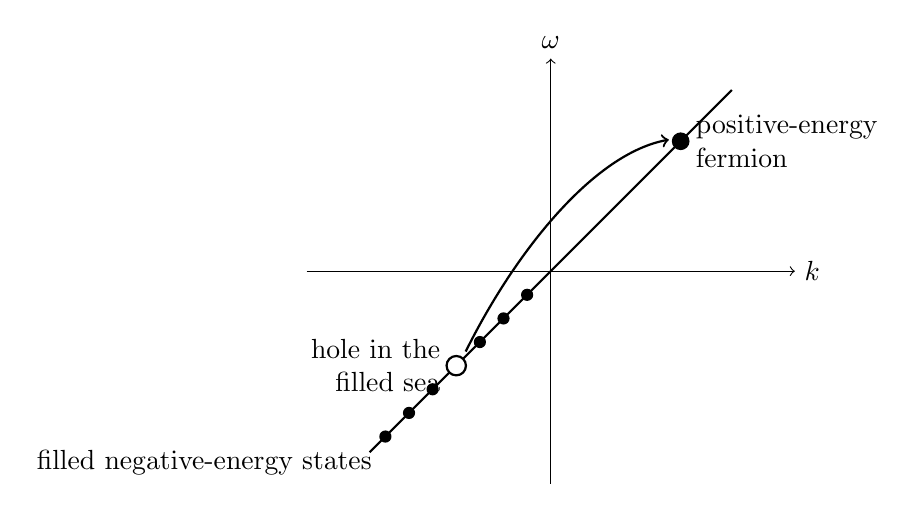
\begin{tikzpicture}[scale=1.0]
\draw[->] (-3.1,0) -- (3.1,0) node[right] {$k$};
\draw[->] (0,-2.7) -- (0,2.7) node[above] {$\omega$};
\draw[thick] (-2.3,-2.3) -- (2.3,2.3);
\foreach \p in {-2.1,-1.8,-1.5,-1.2,-0.9,-0.6,-0.3}{
  \fill (\p,\p) circle (2.2pt);
}
\draw[fill=white,thick] (-1.2,-1.2) circle (3.5pt);
\fill (1.65,1.65) circle (3.2pt);
\draw[->,thick] (-1.08,-1.02) .. controls (-0.45,0.25) and (0.55,1.5) .. (1.5,1.67);
\node[left,align=right] at (-1.28,-1.2) {hole in the\\filled sea};
\node[right,align=left] at (1.72,1.65) {positive-energy\\fermion};
\node[below left] at (-2.15,-2.15) {filled negative-energy states};
\end{tikzpicture}%
}
\caption{満たされた負エネルギー海と、1つのフェルミオンを正エネルギーへ励起することによって形成された励起。}
\end{figure}

最も単純な励起は、負エネルギー海から1つのフェルミオンを取り除き、それを正エネルギー状態に置く。励起されたフェルミオンは通常の正エネルギーの粒子である。海に残された空席は第2の励起であり、空孔である。取り除かれたフェルミオンが負電荷を帯びているならば、空孔は正電荷を帯びている。

この一分枝の例では、空孔もまた正の運動量を持つ。失われたフェルミオンが運動量\(k_-<0\)の状態を占めていたならば、それを取り除くことは全運動量を
\begin{equation}
p_{\mathrm{hole}}=-k_->0.
\end{equation}
だけ変化させる。それは負の運動量の不足である。したがって、励起は正エネルギーで負電荷のフェルミオンと、正エネルギーで正電荷の空孔からなる。両方とも正の運動量を運び、\(\omega=k\)分枝上では、両方とも右へ移動する。

完全な電子理論では、正電荷の空孔は陽電子である。ディラックは当初、空孔を陽子と同定することを考えた。この構成は、粒子とその反粒子が同じ質量を持つことを要求する。空孔は電子の質量と同じで反対の電荷を持つ別個の粒子である。これが、負エネルギー・スペクトルが導いた基本的な粒子--反粒子解釈である。

同じ救済策をボソンに適用することはできない。ボソン状態は任意個の粒子を許容するため、負エネルギーの準位を一度だけ埋めてそれ以上の占有を阻止する方法はない。より多くのボソンをその準位に加え続けることが常に可能であり、エネルギーは何度でも低下する：
\begin{equation}
\begin{aligned}
\text{fermionic mode: }&n=0\ \text{or}\ 1,\\
\text{bosonic mode: }&n=0,1,2,\ldots .
\end{aligned}
\end{equation}
提案されたボソン系には依然として基底状態が存在しないであろう。この初等的な構成において、埋め尽くされた海の安定性はまさにフェルミオン的排他性に依存している。

この一次元方程式はディラック方程式の玩具版にすぎない。その場は質量がなく、光速で運動し、一方向にのみ伝播する。より完全なディラック方程式は、欠けている運動の方向と相対論的粒子構造の残りの部分を扱わなければならない。そのより完全な方程式は、ボソン場に対する反粒子の取り扱いとともに、後回しにされる。